\begin{table*}[t]
            \small
            \renewcommand{\arraystretch}{1.7}
            \begin{center}
            \caption{\label{tab: Guide Personas} Our guide’s three personas: the human, the guide dog, and the robot. The voices mentioned for each persona (Alloy, Nova, and Onyx) are OpenAI’s default TTS voices \cite{openai-tts}. Audio samples of each voice can be found at the cited link. The personality prompts were sent to GPT-4 to shape the guide's responses (see supplemental materials). All columns are based on our previous designs from Collins et al. \cite{collins2024ai}, except for Speech Sample, which was produced by our current implementation of the AI guide.}
                \begin{tabular}{|P{1cm} | M{2cm} | P{2cm} | P{2cm} | P{2cm} | P{2cm} |P{3.2cm} |}
                    \hline
                    \textbf{Persona} & \textbf{Guide Avatar} & \textbf{Guide Description} &
                    \textbf{Guide Movement} &
                    \textbf{Voice + Speech Characteristics} &
                    \textbf{Personality Prompt} & \textbf{Speech Sample} \\ \hline
                    \textbf{Human} & \raisebox{-\totalheight}{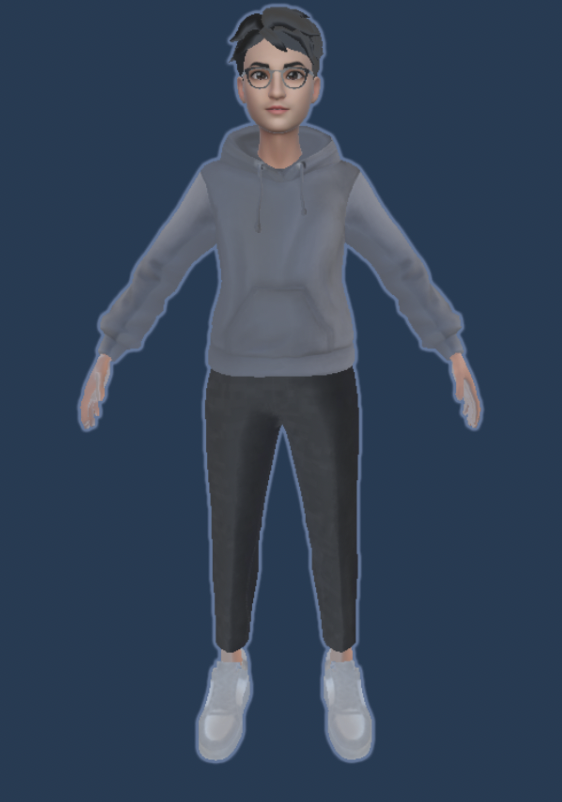
\includegraphics[width=1.8cm, height=2.3cm]{human_guide.png}} & An androgynous human with short black hair and glasses, wearing a gray hoodie and black pants. & Follows behind the user from an arm’s length away. Footstep sound effects indicate movement. & \textit{Alloy,} androgynous voice, medium formality (some jokes, casual speech), averages 101.2 words per response & Warm, friendly, but still professional sighted guide & \textit{The scene around you is a simple, geometric landscape composed of distinctive objects. To your right stands the Tall Building, a towering yellow cube that rises high above the rest…} \\
                    \hline
                    \textbf{Guide Dog} & \raisebox{-\totalheight}{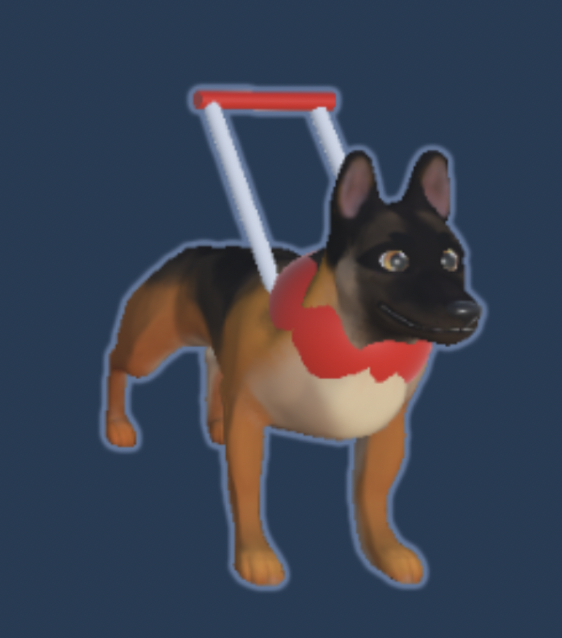
\includegraphics[width=2cm, height=2cm]{dog_guide.png}} & German-shepherd with black and brown fur, wearing a bright-red guide dog harness. & Walks beside the user on their left side. The sounds of panting and paws scratching the floor indicate movement. & \textit{Nova,} feminine voice, low formality (uses slang, jokes, and casual speech), averages 185.4 words per response & Very friendly, excited companion who is eager to please who you’re talking to & \textit{What an exciting world we're in! To your right stands the impressive Tall Building, reaching up high with its yellow facade…} \\
                    \hline
                    \textbf{Robot} & \raisebox{-\totalheight}{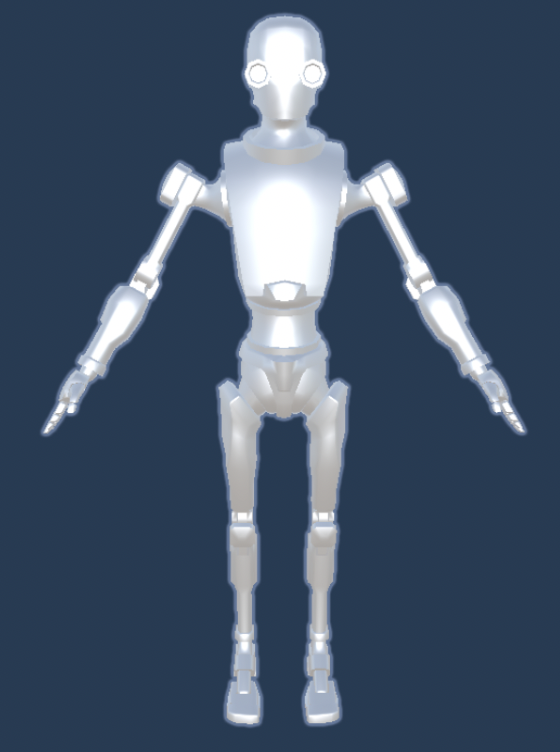
\includegraphics[width=1.8cm, height=2.3cm]{robot_guide.png}} & A shiny, silver robot that is humanoid in stature, with a masculine frame. & Follows behind the user from an arm’s length away. Creaking machinery sound effects indicate movement. & \textit{Onyx,} masculine voice, high formality (speaks entirely in proper sentences, no casual speech), averages 91.2 words per response & Formal and assertive assistant who talks like a robot & \textit{Affirmative. The area around you is composed of geometric shapes and structures. Directly to your right lies the Tall Building…} \\
                    \hline
                \end{tabular}
                \newline\newline
                \Description{Information about three different guide personas. Contains all textual content, aside from the three images of the persona's avatars in the column "Guide Avatar." Each avatar is described in the following column "Guide Description."}
            \end{center}
        \end{table*}